\section{Attack Design}

\subsection{Overview}
 In this paper, we investigate the feasibility of spoofing the face authentication system using a public 2D photo of a legitimate user by bypassing its 3D liveness detection module. 
 To guarantee an effective and robust spoofing attack in the real world, it is important to address the following  challenges:

\begin{itemize}
	\item \textbf{Challenge 1:} 
	How to estimate the depth information from a public 2D photo of the victim?
	\item \textbf{Challenge 2:} 
	How to convert the estimated depth into a structured light scatter pattern such that it can be received and regarded as real depth information by the system?
	\item \textbf{Challenge 3:} 
	How to spoof the system if it employs both RGB and depth liveness detection?

\end{itemize}

To address these challenges, we design the \texttt{DepthFake} attack consisting of three steps as shown in Fig.~\ref{overview}. 
The \textbf{Depth Estimation} module detects and extracts the face region from a 2D public photo of the victim, and estimates its depth information through a CNN-based deep learning model. 
The \textbf{Depth Forgery} module extracts and denoises the template scatter pattern of the target depth camera by using local-threshold filtering, maps the estimated depth  into the template scatter pattern, and projects it to forge a real-world depth image by using an infrared projector. 
The \textbf{RGB-D Alignment} module spoofs the RGB and depth liveness detection 
in the meantime by first generating a RGB adversarial photo using an evolutionary strategy and then physically aligning the forged RGB image and the projected scatter pattern to launch a uniform RGB-D attack.
In the following sections, we present these attack building blocks in detail.

\begin{figure}[pt]
	\centering
	\subfigure[Front face]{
		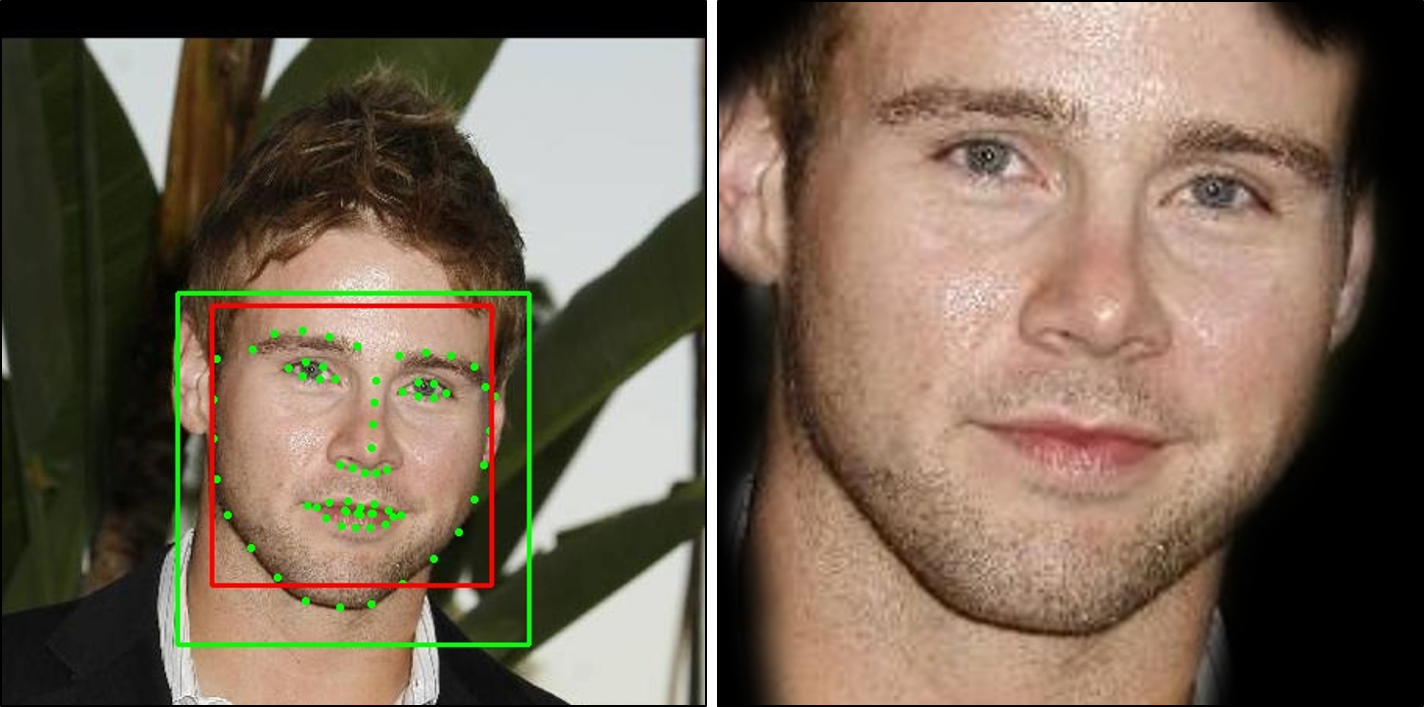
\includegraphics[width=0.22\textwidth]{figures/estimation/frontface.png} 
	}
	\subfigure[Side face]{
		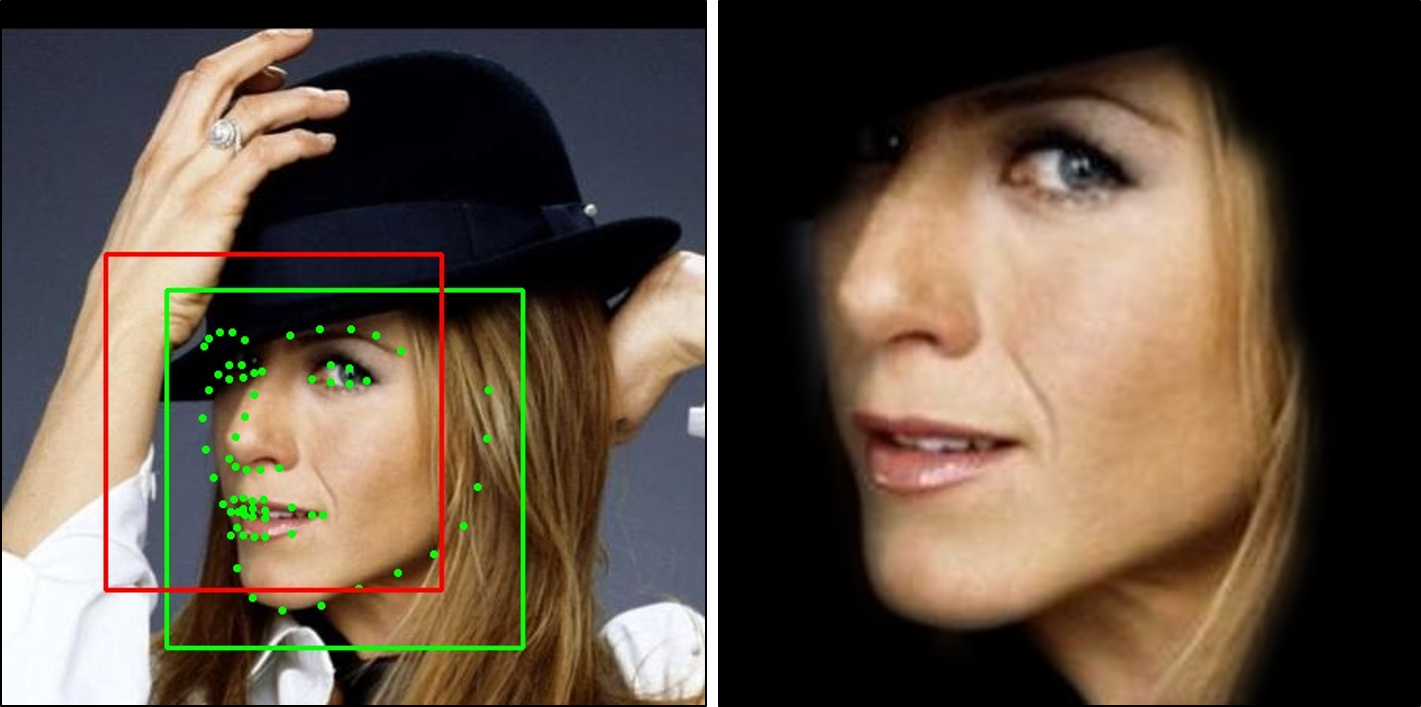
\includegraphics[width=0.22\textwidth]{figures/estimation/sideface.png} 
	}
	\vspace{-0.1in}
	\caption{Face region extraction from the photo of victims. (a) is an example of front-face, (b) is an example of side-face. The green points are the 68 feature landmark points. The red and green bounding-boxes represent the face region detected by Dlib and our method respectively.}
	\label{face_extraction}
	\vspace{-0.15in}
\end{figure}

\subsection{Depth Estimation}
To spoof 3D face authentication systems using a  public photo, we first estimate and reconstruct a depth image of the victim from his 2D photo. In general, the depth estimation has two steps: (1) Face extraction that extracts the victim's face region from his/her 2D photo to eliminate the influence of background elements, and (2) Depth estimation that estimates the depth information of the face region and generates a pixel-to-pixel depth image by using a CNN model.

\subsubsection{Face Extraction}
To estimate user depth information via a public photo, we first  detect and crop the face region to  improve the processing efficiency.

\textbf{Face Detection.} For face detection, a commonly-used  tool is the Dlib Library~\cite{dlib09}. However, using this tool alone cannot detect the  face region completely, especially the side one, as shown in the red bounding box in Fig.~\ref{face_extraction}.
To obtain the face region precisely, we improve the face detection function in the  Dlib Library by considering the following two aspects: (1) the size of the bounding box shall be appropriate to contain the entire face including the contours, and (2) the face shall  locate at the center of the bounding box to reduce background elements. To achieve it, we first utilize the shape predictor of the Dlib Library to landmark 68 key feature points of the face. Then, we use these feature points to determine the  coordinates of the center point and the side length of the bounding box such that the face can be entirely contained and located in the center of the bounding box. 
%In addition, we enlarge the bounding box with $1.2\times$ to cover the whole face region.

As shown in Fig.~\ref{face_extraction},  our face detection method can extract the face region precisely and completely for both front and side face images.

\textbf{Face Region Cropping.} 
After extracting the face region from the victim's photo, we crop and resize it to 224 $\times$ 224 pixels, i.e., the default input size for the following depth estimation model.
%To further remove the background elements, we extract the precise face region by utilizing a face segmentation method ~\cite{nirkin2018_faceswap}. 

\subsubsection{CNN-based Face Depth Estimation}
To estimate the depth information from the cropped face region, we then propose a pixel-to-pixel method based on convolution neural networks (CNNs). We employs the UNet~\cite{ronneberger2015u} as our model architecture. It uses the  ResNet-50~\cite{he2016deep} as the encoder to reduce a 224 $\times$ 224 input image into a 7 $\times$ 7 embedding feature map, and uses a decoder formed by 5 transposed convolutional layers and 10 convolutional layers to reconstruct the feature map into a 224 $\times$ 224 depth image, where each pixel represents the absolute value of the depth.  Then, we design the loss function to optimize the aforementioned estimation process.


\begin{figure}[!t]
	\centering
	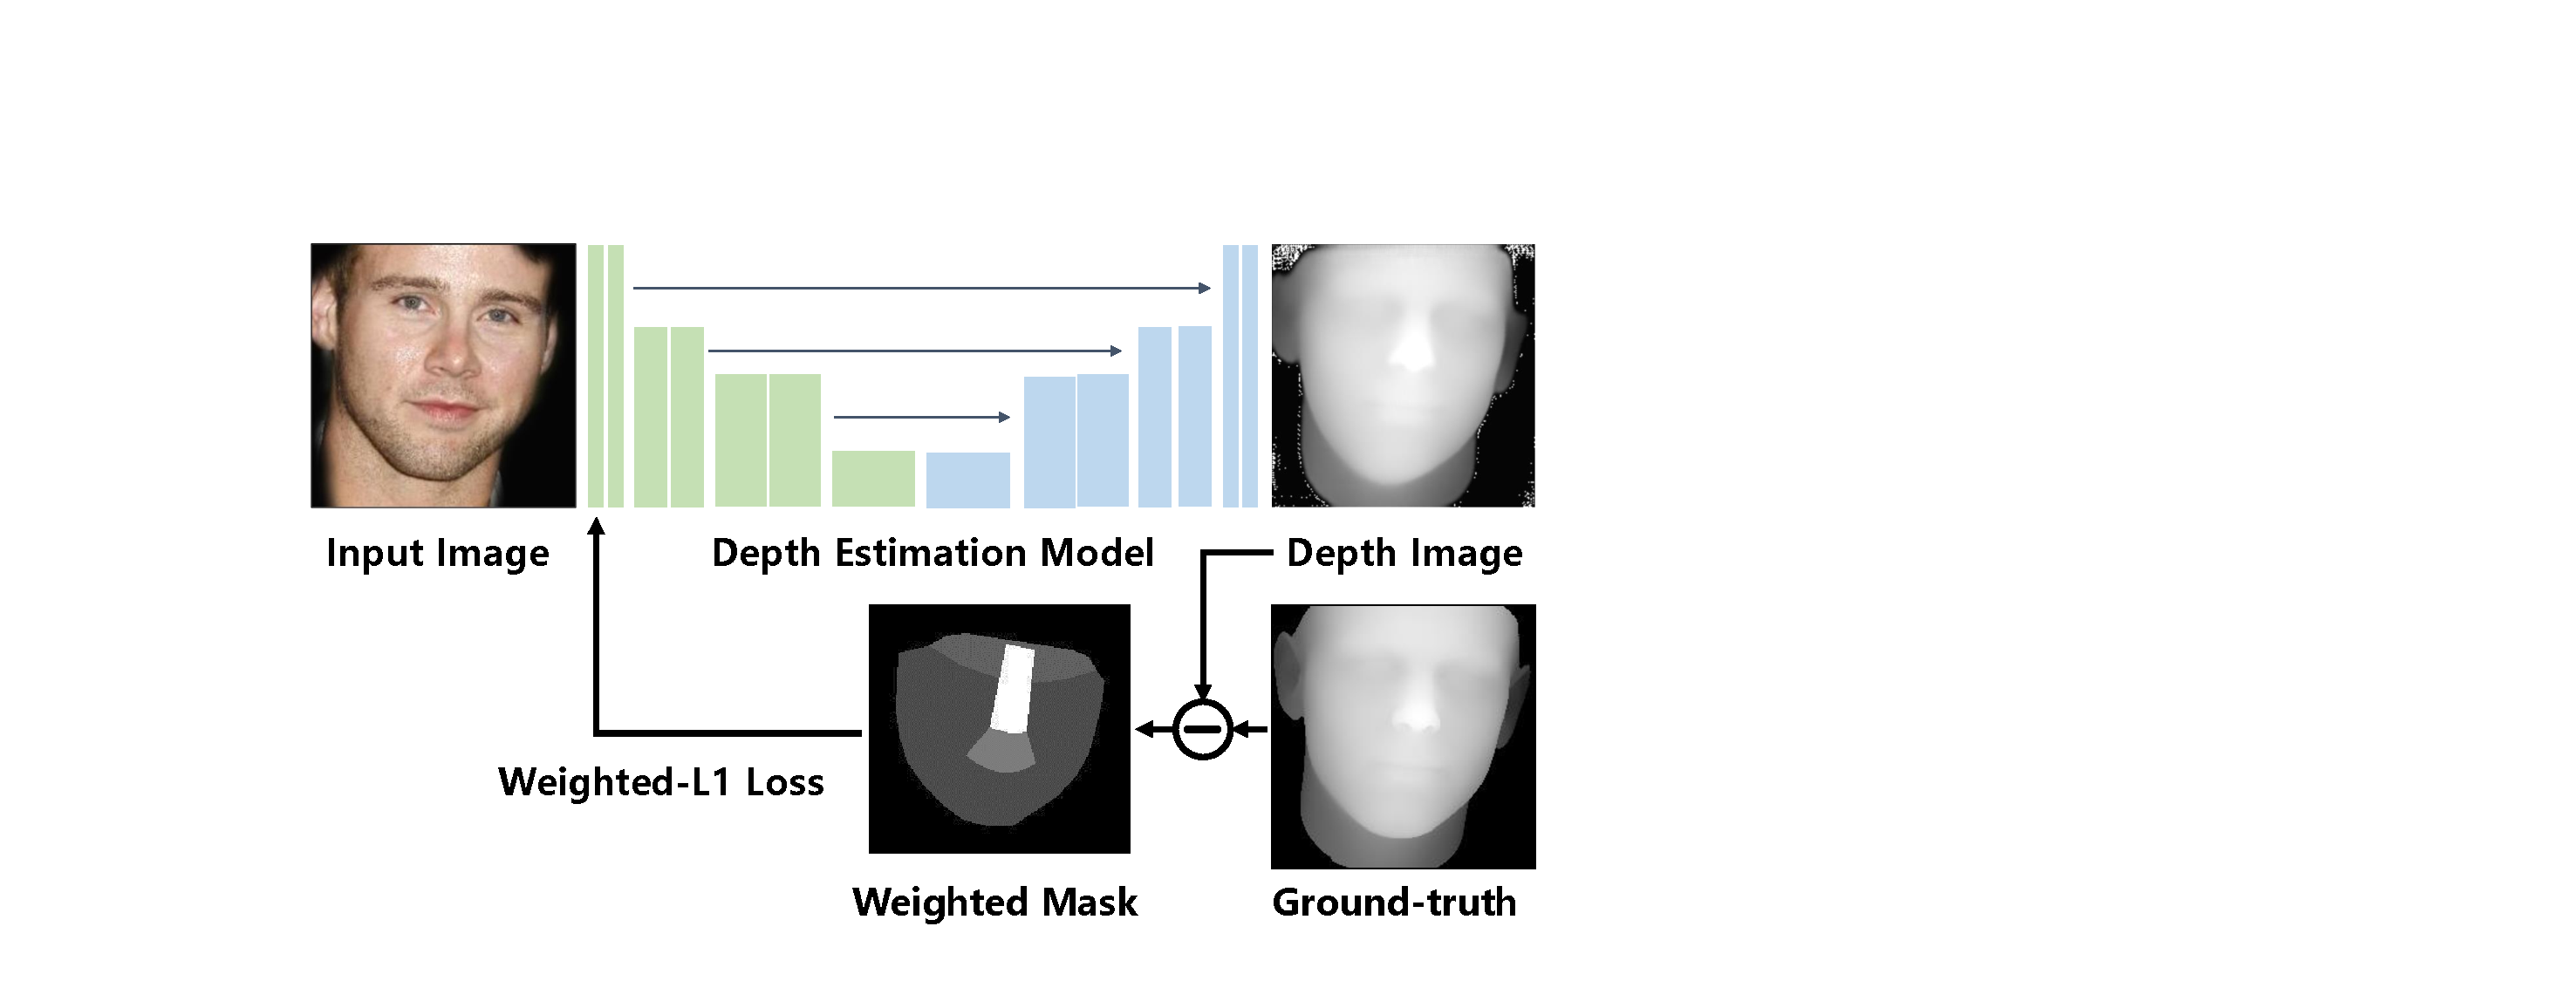
\includegraphics[width=0.47\textwidth]{figures/model_architecture_1.pdf} 
	\vspace{-0.15in}
	\caption{Model architecture for depth estimation.The depth estimation model generate the depth image from the input RGB image, and use its weighted mask to build the loss function.}
	\label{model_architecture}
	\vspace{-0.15in}
\end{figure}

\textbf{Loss Function Design.} In general, U-Net utilizes the L1 Loss as the loss function to optimize the depth estimation task. However, the L1 Loss treats all pixels in the image equally, leading to depth estimation errors in  regions such as  noses, eyes and mouths. Those regions, however, are important in feature representation and depth reconstruction.  To address it, we propose to employ a weighted L1 Loss, which assigns more weights to the central parts of the face (i.e., the nose, eyes and mouth) compared with other regions. Specifically,  we use the landmark feature points to locate the key regions and assign different weights to them to form a weight mask. As shown in Fig.~\ref{model_architecture},  we assign a weight of  2 for the nose region, 1.5 for the eye and mouth regions, 1 for other face regions, and 0 for non-face regions. In this way, we make the model pay more attention to reconstructing the depth of the nose, eyes and mouth regions. 
The proposed weighted L1 Loss is as follows:
\begin{equation}
	Weight{-}L1=\frac{1}{N}\sum_{i=1}^{N} \lvert y_i - f(x_i) \rvert \times WeightMask
	\label{weigted_loss}
\end{equation}
where $x$ and $y$ are the input image and the ground-truth depth image,  and$f(\cdot)$ is the depth estimation model.

\textbf{Model Training.}
We use the 300W-3D face dataset~\cite{zhu2016face} as the training dataset, use the Texas 3DFR dataset~\cite{gupta2010anthropometric, gupta2010texas} as the testing dataset, and employ Adam with a learning rate of $1e{-}5$  as the optimizer to train the depth estimation model.  An illustration of the depth estimation result is shown in Fig.~\ref{estimation_result}. Compared to the ground-truth image and its 3D mesh plot, the depth image estimated from the 2D image shows a normalized mean error less than $2\%$, and can spoof the depth-based liveness detection module in commercial face authentication SDKs (i.e., Tencent, Baidu, and 3DiVi) with nearly $100\%$ attack success rates.
%We also leverage the estimated depth images into the liveness detection module in commercial face authentication SDKs (i.e., Tencent, Baidu, and 3DiVi) and get both $100\%$ attack success rates in the testing dataset.

%At training phase, we use the 300W-3D face dataset~\cite{zhu2016face} which contains images of different genders, human races, lighting conditions, and face angles as our training dataset. As for the testing dataset, we choose the Texas 3DFR dataset~\cite{gupta2010anthropometric, gupta2010texas} whose ground-truth depth images are captured by depth sensors in the real world. Before training, we pre-process the images in the dataset using the face extraction method, and ensure that the input images have removed the background noises. During training, we use Adam as the optimizer with a learning rate at $1e{-}5$ and train the model in an NVIDIA 2080 Ti GPU. Besides, we evaluate the model after each training epoch by employing Normalized Mean Error (NME) in the testing dataset and choose the model that has the best performance as our depth estimation model.

%An example of the results using our depth estimation method is shown in Fig.~\ref{estimation_result}. Compared to the ground-truth image and its 3D mesh plot, our method can successfully reconstruct the depth information from the target 2D image with a minimal error. 
%To evaluate the effectiveness of our depth estimation method within the different individuals, we conduct experiments on our testing dataset which contains 105 individuals with different gender, ethnicity, and facial expression. We achieve the result of $1.90\%$ as evaluate metric NME in the testing dataset. It is better than other face reconstruction methods such as PRNet which gets $5.51\%$ of NME in the same testing dataset. The reason is that such methods rely on the 3D Morphable Model (3DMM) to reconstruct the face, but the output images are all normalized in the 3DMM parameter space and do not accurately represent the true depth information of the face.



\begin{figure}[!t]
	\centering
	\subfigure[Ground truth]{
		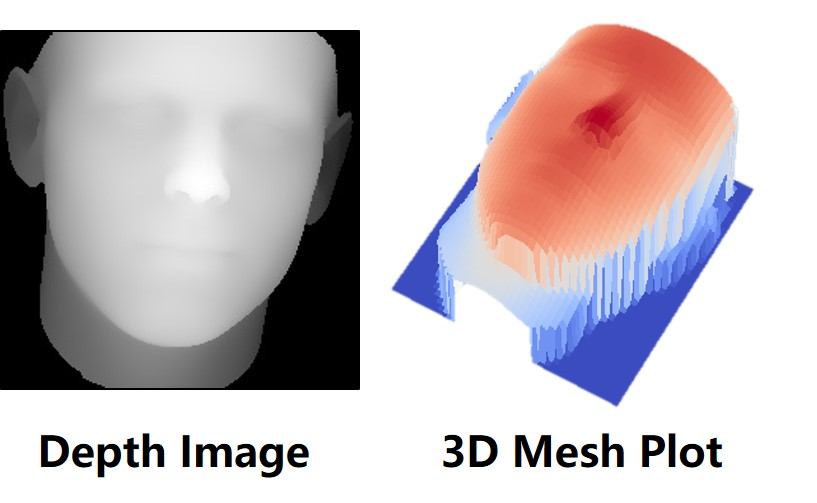
\includegraphics[width=0.22\textwidth]{figures/estimation/pred_results_groundtruth.jpg} 
	}
	\subfigure[Estimation result]{
		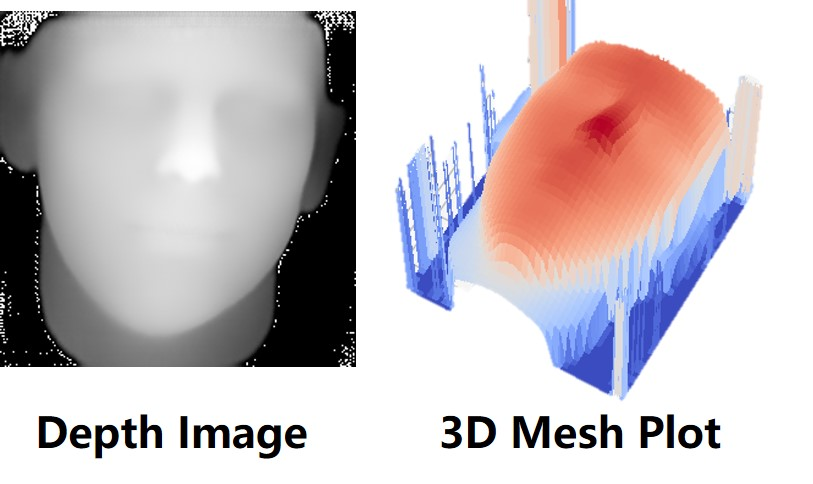
\includegraphics[width=0.22\textwidth]{figures/estimation/pred_results_pred.jpg} 
	}
	\vspace{-0.1in}
	\caption{Depth estimation results. (a) is the ground-truth depth image and its 3D mesh plot of the target image. (b) is the estimated depth image and its 3D mesh plot from our model.}
	\label{estimation_result}
\vspace{-0.15in}
\end{figure}

\subsection{Depth Forgery}
The structured light depth camera calculates the depth information by measuring the displacements of scatter points between the template scatter pattern and the reflected one.  To spoof it, the adversary shall modulate the estimated depth information into the template scatter pattern such that it can be captured and accepted by the depth camera.  
To achieve it, we propose a depth forgery method consisting of two steps: (1) extracting the template scatter pattern of the victim camera, and (2) modulating the estimated depth image into the template scatter pattern to form the spoofing scatter pattern. 
%For a real-world attacker, she need to deploy the depth image in the physical world. Thus, we propose a depth forgery method based on the imaging mechanism of structured light camera, which consists of three steps: (1) extracting the template scatter of the camera, (2) mapping the estimated depth image into the scatter pattern and projecting the scatter pattern and ensure it can be captured by camera to form the forgery depth image we designed. In the following, we introduce our depth forgery method in detail.

\subsubsection{Template Scatter Extraction}
Different structured light depth cameras use different template scatter patterns. Thus, we shall first obtain the template scatter pattern of the victim camera. 
A naive but effective method is to use an infrared camera to capture an image towards it and extract the template scatter pattern from the captured infrared image. However, the raw infrared image usually suffers from various noises, rendering the extracted template scatter pattern not precise and thus  introducing extra errors in depth forgery. To extract a clear and precise template scatter pattern, we propose an image noise reduction method called local-threshold filtering. 

Since the scatter point is usually the brightest in its surrounding neighborhood while the noises can be dim, we can use the non-maximum suppression (NMS)~\cite{girshick2014rich} to remove the background noises. NMS is a mathematical method for picking the maximum value within an array while suppressing other values. For instance, if we have an array $A$ as $\left \{A_1, A_2, ...,A_n \right \}$ and the maximum value of $A$ is $A_{max}$, the NMS algorithm will only retain $A_k$ and set the other value to 0 as follows:
\begin{equation}
	\textbf{NMS}(A)=\left \{0, 0, ..., A_{max},...,0 \right \}\label{nms_1}
\end{equation}

To employ NMS for image processing, we extend the one-dimensional NMS into two-dimensional by using the sliding window. Specifically, we extract the pixels with the maximum grayscale value within each small region.
Since a scatter may cross more than one pixel when captured by the infrared camera, the pixels around the maximum value pixel may also have  larger grayscale values than other pixels. 
To ensure the precise of the extracted template scatter pattern, we retain the pixels whose grayscale value larger than a threshold and set the others to 0. We set the threshold dramatically with the following equation since the grayscale of the scatter points in the sliding window is related to the background brightness.
\begin{equation}
	threshold = -0.001(p_{max})^2 + 1.0001 p_{max}\label{nms_2}
\end{equation}
where $p_{max} \in \left [ 0, 255 \right ]$ is the maximum value in the sliding window. An illustration of the extracted template scatter pattern is shown in Fig.~\ref{template_extraction}.


\begin{figure}[!t]
	\centering
	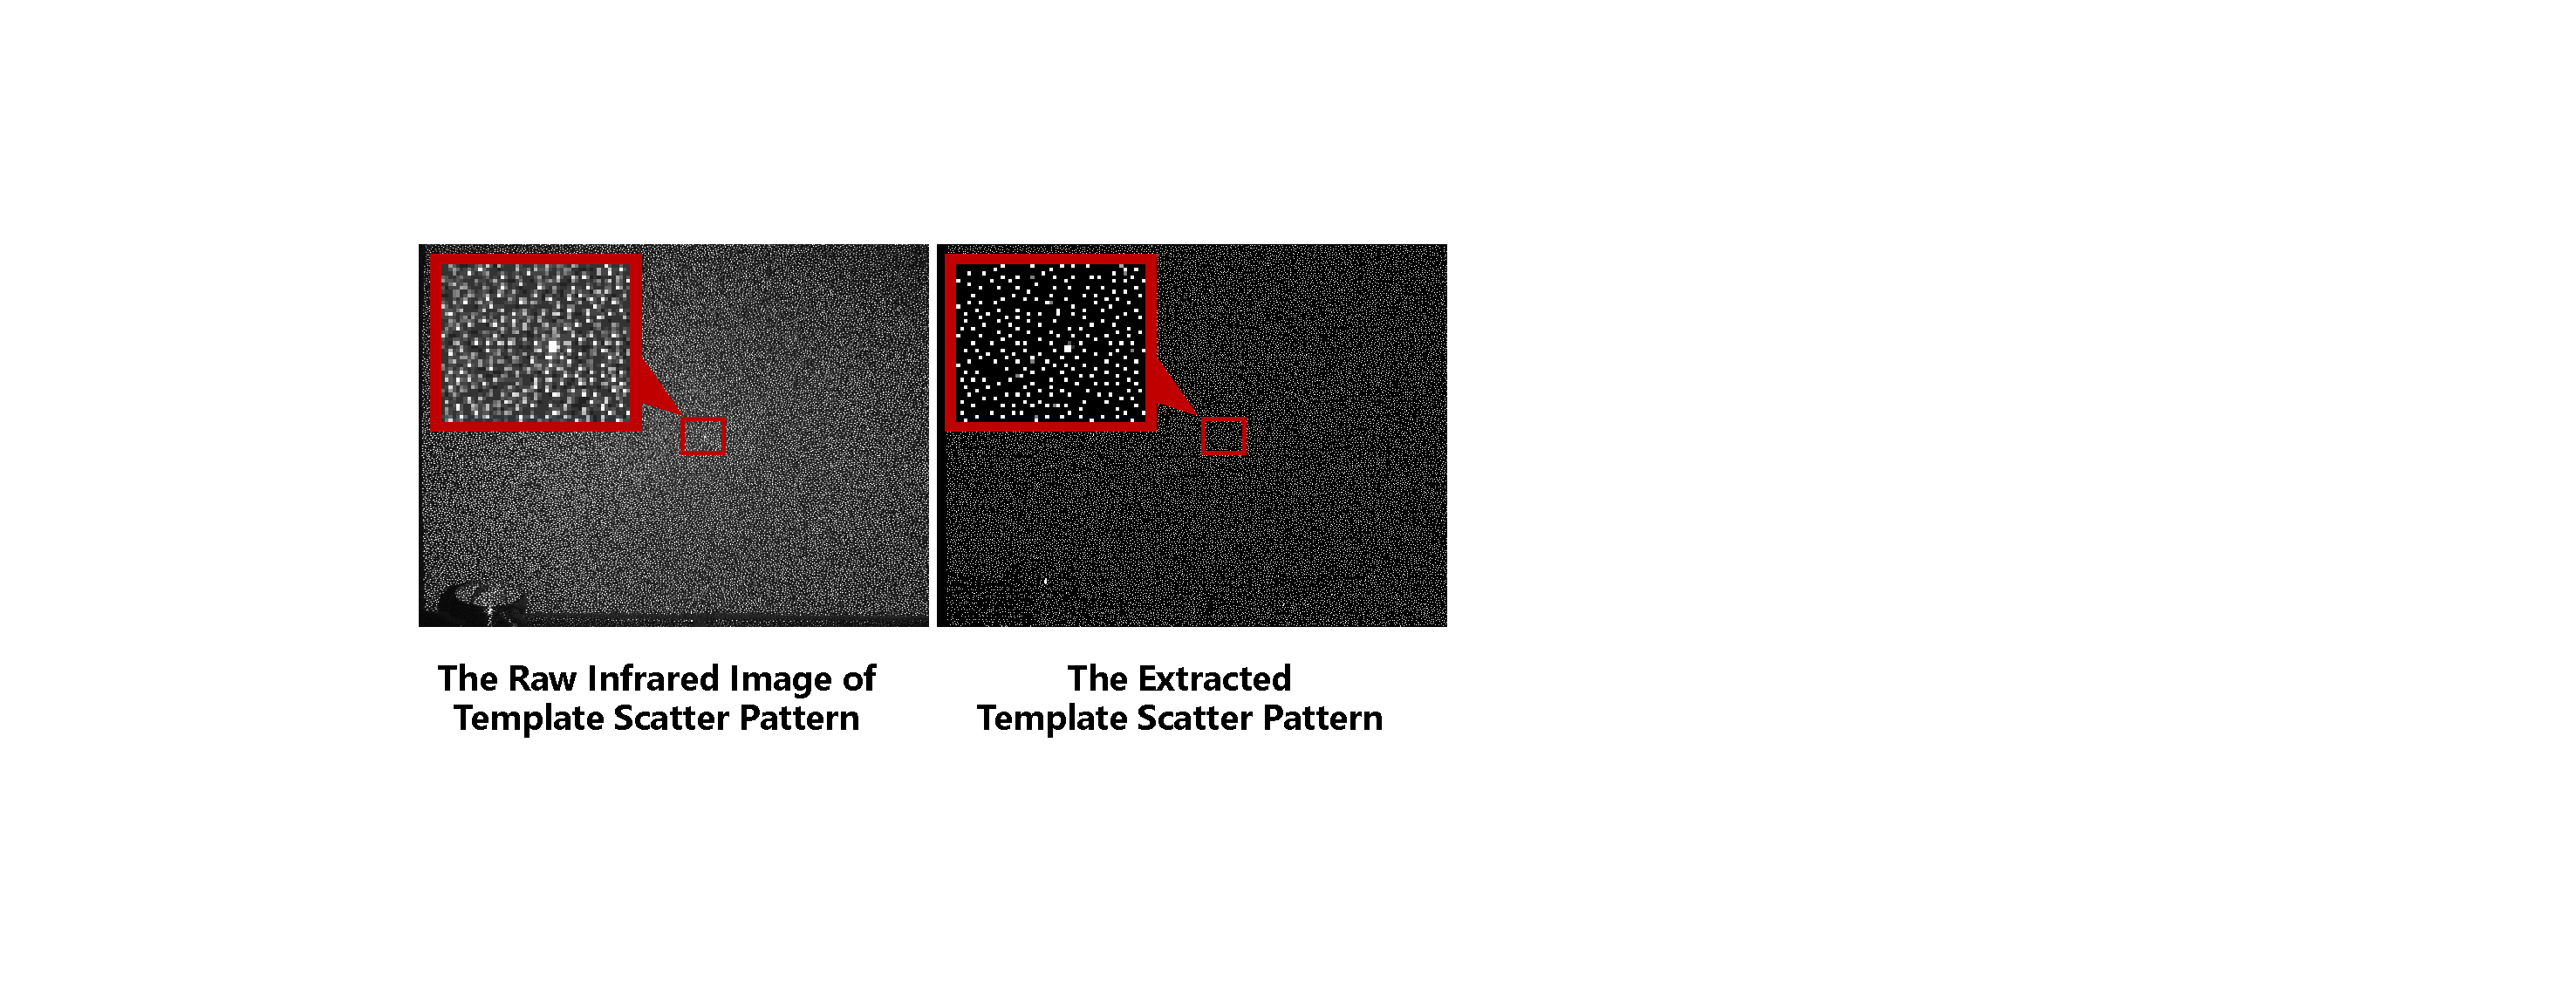
\includegraphics[width=0.48\textwidth]{figures/template_extraction.pdf} 
	\vspace{-0.15in}
	\caption{Template Extraction. Images from left to right are the raw infrared image of the template scatter pattern and the extracted template scatter pattern.}
	\label{template_extraction}
	\vspace{-0.15in}
\end{figure}


\subsubsection{Depth-to-Scatter Modulation Strategy}
Then, we modulate the estimated depth information into the extracted template scatter pattern by shifting the locations of its scatter points. 
%changing the different displacements of the scatter points on the template scatter pattern. As we have obtained the template scatter pattern and the estimated depth image, we then propose a depth-to-scatter modulation strategy to generate the diesired scatter pattern.
Two key questions here are, for each scatter point in the template: (1) What's its depth value? (2) What is  the corresponding displacement that represents the depth value?

 
%match the depth information and the template such that match each scatter point on the template  to their corresponding depth information and model the modulation process.Then, we build the mapping function from depth to scatter points' displacements, estimate its parameters and use it to generate the desired scatter pattern.

%The depth forgery in the real world rely on the desired scatter pattern. Therefore, the attacker need to transfer the digital estimated depth image into the scatter pattern, then project it and make the depth camera to capture a fake depth image. 
%To achieve such a scatter pattern from the digital depth image, we propose a depth-to-scatter mapping strategy. First, we model the depth forgery process and build the mapping function between the displacements of projected scatter points and the depths. Then, we estimate the parameters of the mapping function. Finally, we convert the whole depth image into the scatter pattern and ensure the camera can capture it to generate the forgery depth.

For the first question, we address it by coordinate alignment. We first extract the coordinates of each scatter point in the template as a set $T = \{(x_1, y_1))_ ..., (x_n, y_n)\}$. Then, based on the coordinates in $T$, we extract the corresponding depth information in the depth map as the set $D = (d_1, ..., d_n)$. 
%Each element in $T$ and $D$ represents the depth information of each scatter point.
The depth-to-scatter modulation process is then can be represented as follows:
\begin{equation}
	S = T + \Phi(D)
	\label{modulation_process}
\end{equation}
where $\Phi(\cdot)$ is the mapping function that converts the depth information to the scatter displacement, and $S$ is the desired scatter pattern.  
Thus, the key to modulate the estimated depth image into the scatter pattern is to build the mapping function $\Phi(\cdot)$. 

\textbf{Mapping Function Modeling.} 
Based on Eq.~\ref{d_cal} in Sec.~\ref{sec:background}, the structured light camera uses the reference depth $d_{ref}$ and the displacement $\Delta x_c$ to calculate the target depth $d_t$. Thus, if a scatter point has a depth value of $d_{t}$, we can obtain its displacement in the camera $\Delta x_c$ as follows:
\begin{equation}
	\Delta x_c = k_cLf_c(\frac{1}{d_{ref}} - \frac{1}{d_t}) 
	\label{d_to_xc}
\end{equation}
where $k_c$ is the number of pixels within a physical length ($1~mm$) in the camera, $L$ is the baseline distance between the camera and the projector, and $f_c$ is the focal length of the camera.

The displacement in the camera $\Delta x_c$ is then can be converted to the displacement in the projector $\Delta x_p$ as follows:
\begin{equation}
	\Delta x_p = \frac{k_pf_p}{k_cf_c}\Delta x_c 
	\label{xc_to_xp}
\end{equation}
where the $f_p$ is the focal length of the projector, and $k_p$ is the number of pixels within a physical length in the projector.

Thus, the mapping function between the depth value $d_t$ and the scatter point displacement $\Delta x_p$ can be expressed as follows:
\begin{equation}
	\Delta x_p = k_pLf_p(\frac{1}{d_{ref}} - \frac{1}{d_t}) 
	\label{xp_to_d}
\end{equation}
Note that parameters $k_p$, $L$, and $f_p$ are related to the attack device (i.e., the infrared projector) only. Thus, the adversary does not need to know any internal parameters about the target device, making the attack more practical in the real world. 

\begin{figure}[!t]
	\centering
	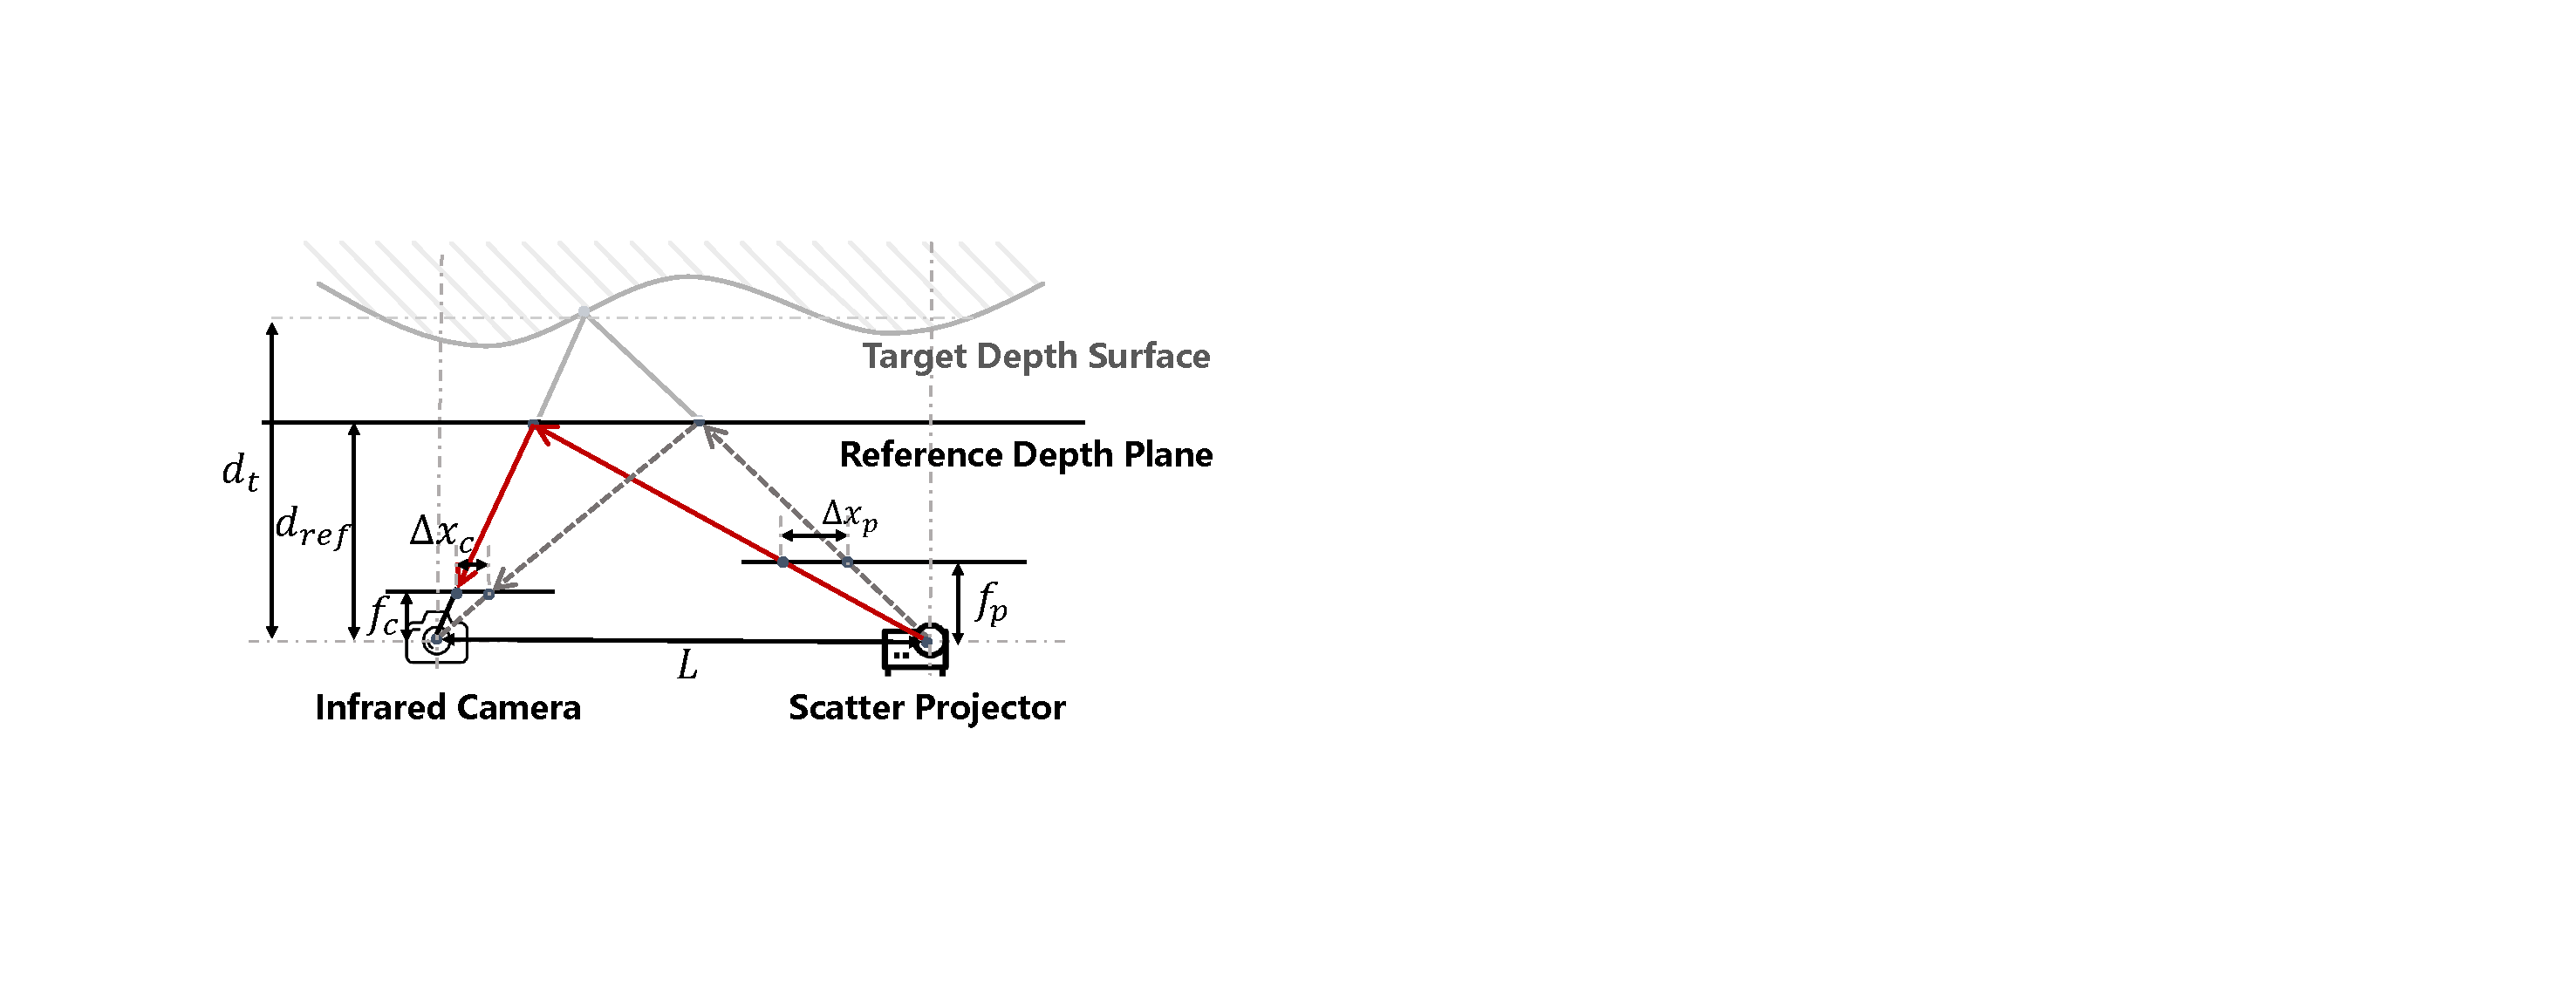
\includegraphics[width=0.48\textwidth]{figures/depth_forgery.pdf} 
	\vspace{-0.1in}
 	\caption{Depth forgery. The scatter point $p$ is shifted by $\Delta x_p$ and projected onto the plane of depth $d_{ref}$ and making it to produce a displacement of $\Delta x_c$ on the imaging plane of the infrared camera. Thus, the camera can be spoofed and calculate the forgery depth $d_t$.}
	\label{depth_forgery}
	\vspace{-0.15in}
\end{figure}


%As shown in Fig.~\ref{depth_forgery}, when the scatter point $p$ located at $x_p$ on the template scatter pattern is projected to the plane of the depth $d_1$, the depth camera will capture it  at $x_{c1}$. However, when we modulate $p$ into the location at $x_p'$, the depth camera then capture it at $x_{c2}$. Since the displacement of $p$ is normally caused by the change of depth, the depth camera will measure the displacements between $x_{c1}$ and $x_{c2}$ and calculate the depth of $p$ as $d_2$, which is the forgery we designed.
%
%Thus, the mapping function $\Phi(\cdot)$ should characterize the relationship between $d_2$, $x_p$ and $x_p'$.
%
%According to the similar triangles, we can derive the relation equations between $x_{p}$, $x_{p}^{'}$ and $d_2$ as follows:
%\begin{equation}
%	x_{p}^{'}=\frac{f_p}{d_1}(L-\frac{x_{c2}d_1}{f_c}) 
%	\label{xp'_cal}
%\end{equation}
%\begin{equation}
%	x_{p}=\frac{f_p}{d_2}(L-\frac{x_{c2}d_2}{f_c})  
%	\label{xp_cal}
%\end{equation}
%where the $L$ is the baseline length,  $f_p$ is the focal length of the projector, the $d_1$ is the depth of plane we project the scatter points and the $d_2$ is the target forgery depth. Based on them, we can get the mapping function as follows:
%\begin{equation}
%	\Phi (d_2) = x_p' - x_p = k_pLf_p(\frac{1}{d_1} - \frac{1}{d_2}) 
%	\label{d_cal2}
%\end{equation}


\textbf{Parameter Estimation.} 
Among the above three parameters, the baseline length $L$ and the focal length of the projector $f_p$ can be measured directly while the number of pixels within a physical length ($k_p$)  cannot.
To address it, we take $k_pLf_p$  as a joint parameter and estimate it integrally.
We record the scatter patterns on planes at depths of $1000mm$, $900mm$, and $800mm$, and use the displacements between them to determine the joint parameter. Specifically, we use the $10 \times 10$ pixels region on the center of the $1000mm$ depth plane as the template scatter pattern. Then, we use the Peak Singal-to-Noise Ratio (PSNR) as a matching function to search for the region with the highest match score and measure the displacement between them. Based on the displacements in different depths, we can estimate the joint parameter $k_pLf_p$. 
For an instance, in this paper, we use a baseline length $L$ of $20mm$, and a reference depth of $1000mm$. By measuring the displacements in depths of $1000mm$, $900mm$, and $800mm$, we can estimate the joint parameter $k_pLf_p$ as 4400 and obtain the mapping function $\Phi(\cdot)$ as follows:
\begin{equation}
		\Phi(d) = 4400 (\frac{1}{1000} - \frac{1}{d}) 
	\label{d_cal3}
\end{equation}
where the $d$ is the target depth.
By modulating the depth information of each scatter point in the set $T$, we can obtain the desired scatter pattern $S$, as shown in Fig.~\ref{depth_mapping}.
%Then, the depth camera can capture this scatter pattern and generate the corresponding forged depth image.

\subsubsection{Projection Correction}
When projecting the forged scatter pattern in practice, there can be a physical distance $L$ between the projector and the victim depth camera, causing projection distortion on the captured scatter pattern. To address it, we employ the perspective transformation~\cite{opencv_library} before projecting, which is commonly used for image correction in computer vision. Based on the perspective transformation function shown in Eq.~\ref{align_2}, we capture both the origin and distorted scatter patterns, select four vertices of the face bounding box as the reference points, and compute the parameter matrix by comparing the pixel offsets between each pair of the vertices.
\begin{equation}
	\begin{bmatrix} \tilde{x} & \tilde{y} & \tilde{w}\end{bmatrix} = \begin{bmatrix} x&y&w\end{bmatrix}
	\begin{bmatrix} 
		a_{11}&a_{11}&a_{11} \\
		a_{21}&a_{22}&a_{23} \\
		a_{31}&a_{32}&a_{33} 
	\end{bmatrix}
	\label{align_2}
\end{equation}
where ($x$, $y$) is the point in the original image, and $w = 1$. 
Then, we use Eq.~\ref{align_3} to compensate for the origin scatter pattern to ensure the captured one is not distorted.
\begin{equation}
	x^{'} = \frac{\tilde{x}}{\tilde{w}};
	y^{'} = \frac{\tilde{y}}{\tilde{w}}
	\label{align_3}
\end{equation}

%\textbf{Depth-to-Scatter Mapping.} To convert the whole depth image, we first match the depth image to each scatter point , and then calculate their displacements to produce the desired scatter pattern. Specifically, we align the template scatter and the depth image according to the coordinates and find the depth infromation of each scatter point. Then, we apply the mapping function to calculate the displacement of each scatter point.  By shifing each scatter point, we can encode the depth information into the scatter patter.
%
%The process of depth-to-scatter mapping is shown in Fig~\ref{depth_mapping}. Afterwards, we project the desired scatter pattern to the plane of depth $d_1$ to make the depth camera capture it and generate the forgery depth image.


%find the corresponding depth information on the depth image based on the coordinates of each scatter point on the template scatter to get the following list:
%match the pixels' depth information with the scatter points on the the template scatter pattern as follows:
%\begin{equation}
%	\{(s^1, d^1, (x^1, y^1)), ...(s^i, d^i, (x^i, y^i)), ...\}
%	\label{d_match}
%\end{equation}
%where the tuple $(s^i, d^i, (x^i, y^i))$ represents the depth and coordinate position of the scatter point $i$.
%Then, we use the mapping function Eq.~\ref{d_cal2} to calculate the displacement of each scatter point and get the following list:
%\begin{equation}
%	\{(s^1, d^1, (x^{'1}, y^1)), ...(s^i, d^i, (x^{'i}, y^i)), ...\}
%	\label{d_match_2}
%\end{equation}
%where the $(x^{'i}, y^i)$ is the scatter position after mapping. Thus, based on the position of each scatter point, we can obtain the desired scatter pattern.



\begin{figure}[!t]
	\centering
	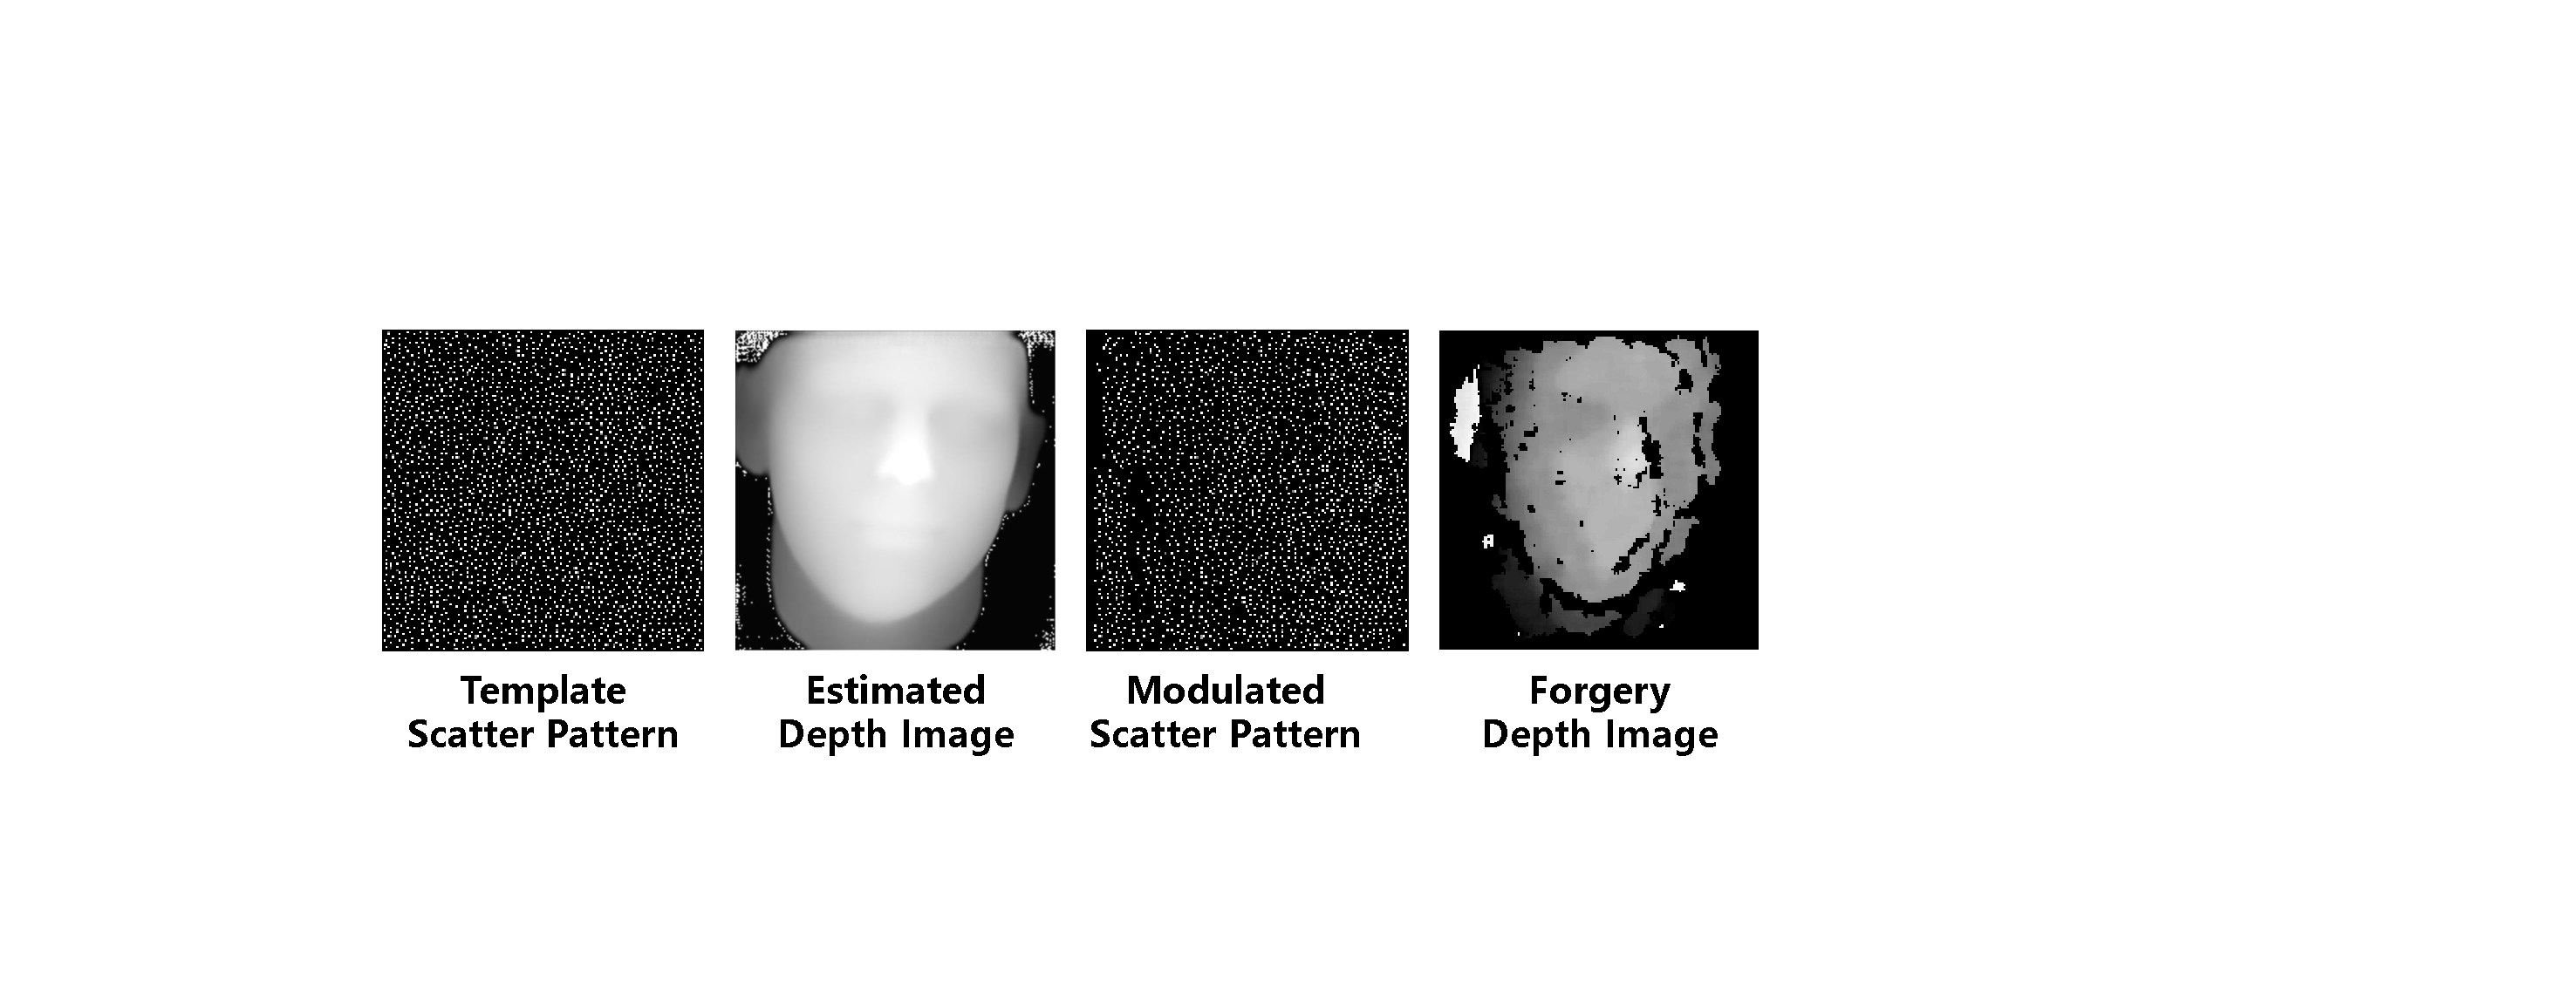
\includegraphics[width=0.48\textwidth]{figures/depth_mapping_1.pdf} 
	\vspace{-0.15in}
	\caption{Depth-to-Scatter Mapping. The digital depth image use the mapping function to convert into a crafted-design scatter pattern, then captured by the depth camera as a physical forgery depth image.}
	\label{depth_mapping}
	\vspace{-0.15in}
\end{figure}


\subsection{RGB-D Alignment}
With the above two attack building blocks, we can spoof depth-based liveness detection. However, some commercial systems may use both RGB and depth for liveness detection. In this case, we shall spoof the RGB-based liveness detection in addition to conducting the depth forgery attack. To achieve this, we propose a black-box optimization algorithm to generate  RGB adversarial examples. Then, we print  and  align it with the forged scatter pattern to launch an uniform RGB-D attack. 
%After depth forgery, we have been able to successfully spoof the 3D liveness detection module in the face authentication system. However, the liveness detection used in commercial products or services extend the 3D liveness detection to RGB-D mode for more security purposes. The reason is that RGB image can provide more color and texture information, and it can help to prevent some simple 3D replay attacks like 3D mask and dummy. Therefore, when the victim face authentication system extend to RGB-D mode, we need to synchronize the RGB attack with the aforementioned depth forgery attack. To achieve this, we first propose a RGB adversarial attack which use the black-box adversarial optimization algorithm and color calibration to generate physical adversarial examples. Then, we align the printed RGB adversarial example with the depth forgery scatter pattern physically to launch a RGB-D synchronized attack.

\begin{figure}[!t]
	\centering
	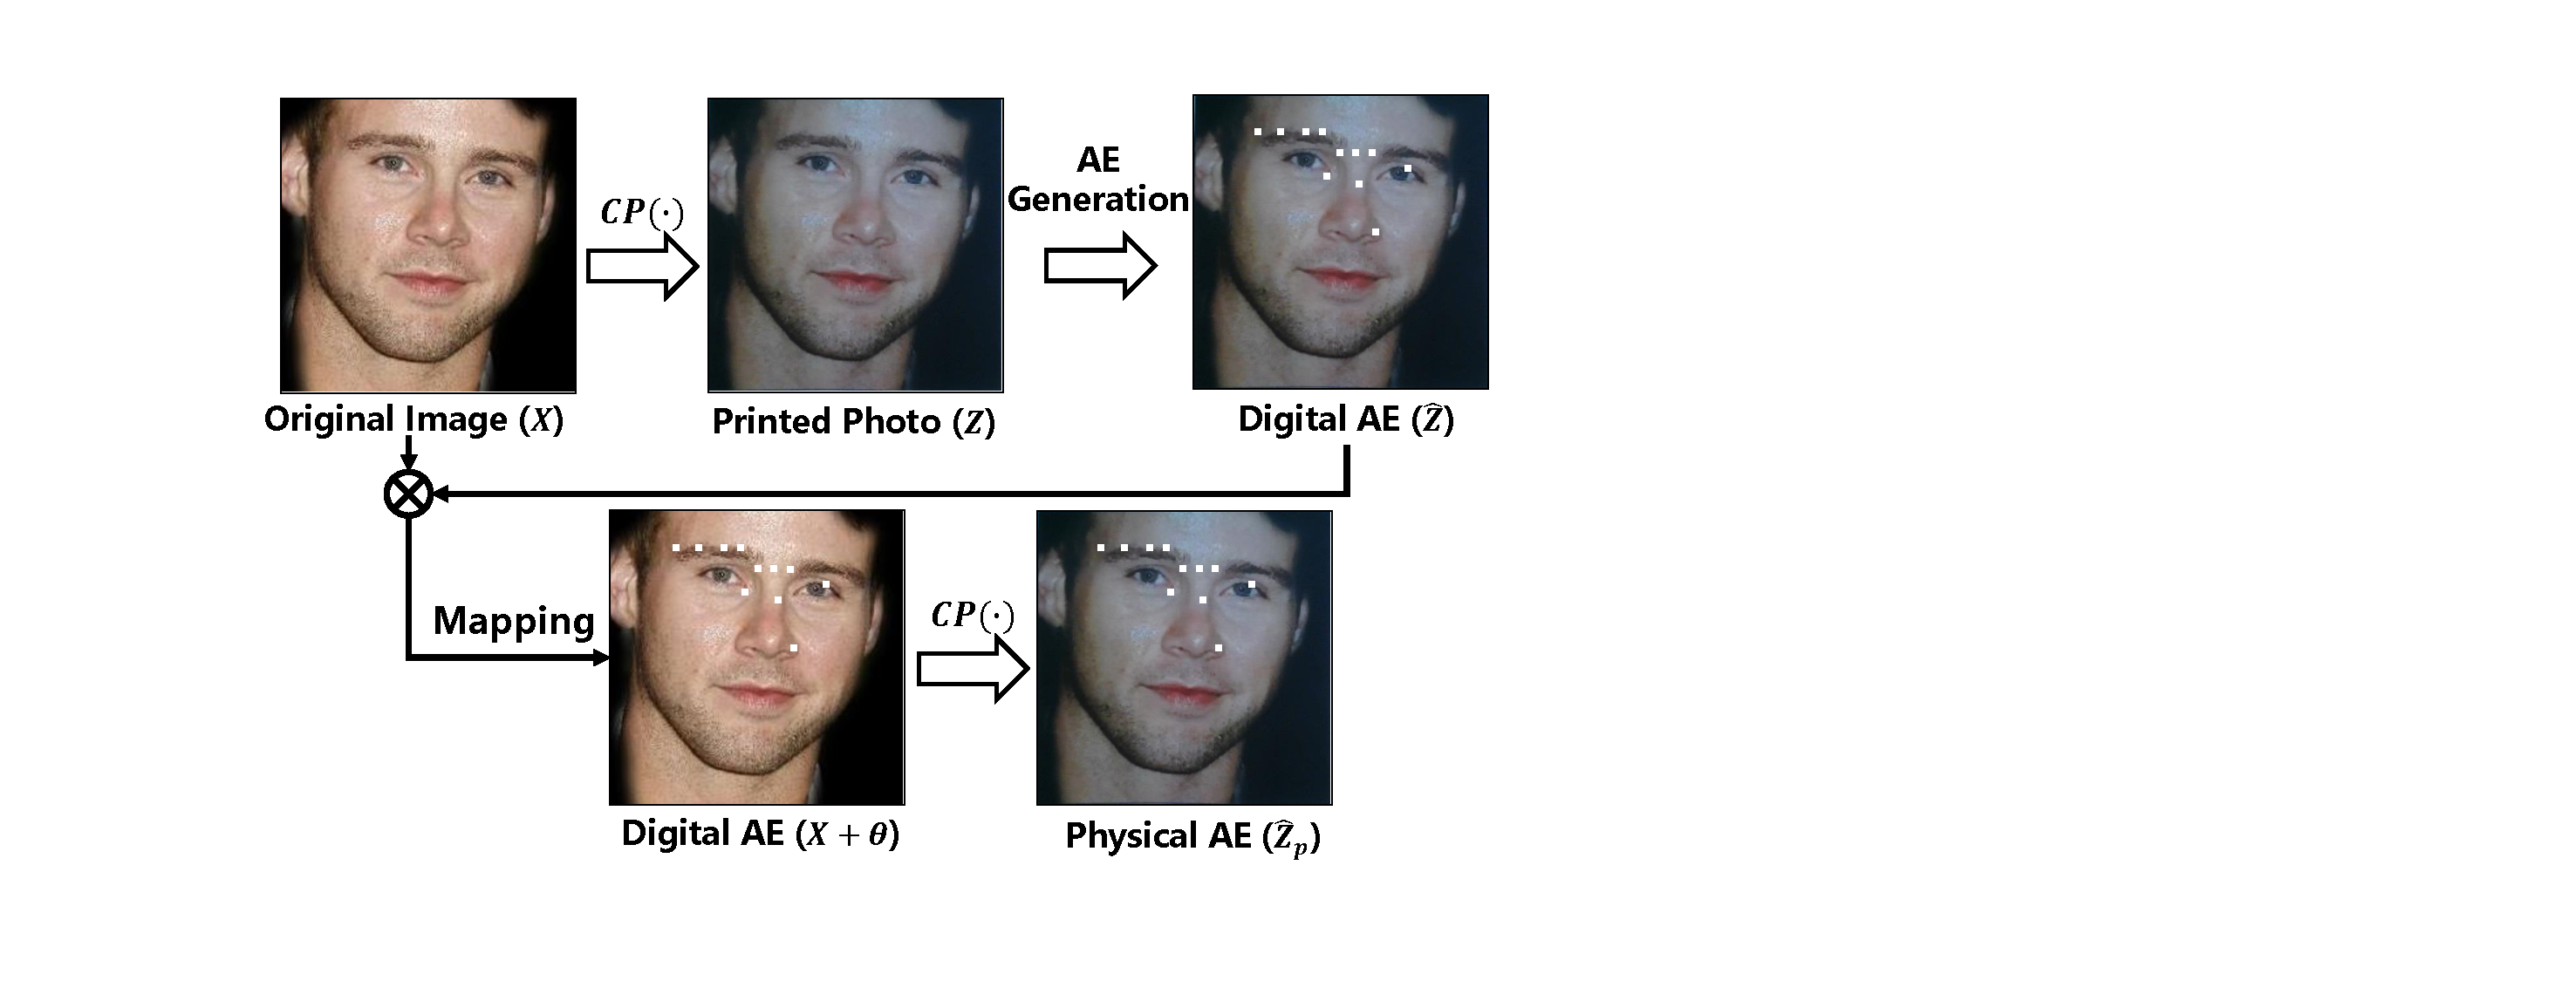
\includegraphics[width=0.45\textwidth]{figures/adv_mapping.pdf} 
	\vspace{-0.1in}
	\caption{The adversarial perturbation $\theta$ generated based on the printed photo $Z$ is applied to the original image $X$ to form the digital adversarial example $\widehat{Z}$, which is then printed and captured as the physical adversarial photo $\widehat{Z}_p$.}
	\label{rgb_mapping}
	\vspace{-0.15in}
\end{figure}

\subsubsection{RGB Adversarial Attack}
As the RGB-based liveness detection usually use CNN as its backbone, we can spoof it with adversarial examples. In general, an adversarial example in our case can be denoted as follows: 
\begin{equation}
	\widehat{Z} = Z+\theta \label{rgb_1}
\end{equation}
where $Z$ is a printed photo detected as ``non-living''  in normal circumstances,  $\theta$ is the optimized adversarial perturbation, and  $\widehat{Z}$ is the adversarial example that can successfully bypass the RGB-based liveness detection in the digital world. However, directly printing the adversarial example as
 an adversarial photo is not enough to guarantee an effective
 attack in the real world, since it suffers from color distortions
 from the printing-capturing process, resulting in a decrease
in the attack effectiveness.  To address it, we first build a printing-capturing
process model and then compensate for the color distortions
in both the printed photo $Z$ and the adversarial perturbation $\theta$.

\textbf{Color Calibration.}
To calibrate the color distortion caused by the printing-capturing process, we first build a model to describe it as follows:
\begin{equation}
	\widehat{Z}_p=C[P(Z+\theta)] =C[P(Z)]+C[P(\theta)]\label{rgb_2}
\end{equation}
where $P(\cdot)$ and $C(\cdot)$ are the abstract transfer functions without loss of generality. Since the printing-capturing process mainly processes each pixel independently~\cite{yin2013image}, we can decouple them. Based on the Eq.~\ref{rgb_2}, we can remove the effect of color distortions on the printed photo $Z$ and the adversarial perturbation $\theta$ separately.

As shown in Fig.~\ref{rgb_mapping}, since the printed photo $Z$ is the original image $X$ after a printing-capturing process, i.e., $Z=C[P(X)]$, we can replace $Z$ with the origin image $X$ in Eq.~\ref{rgb_2} to eliminate the color distortions. For the adversarial perturbation $\theta$, we use white adversarial units instead of pixel-level adversarial perturbations, since the color white does not produce color distortions under the CMYK printing mode. 
By implementing the color calibration, we can get a desired adversarial photo as follows:
\begin{equation}
	\widehat{Z}_p=C[P(X+\theta)] =C[P(X)]+C[P(\theta)]=Z+\theta\label{rgb_3}
\end{equation}

\textbf{Black-box Adversarial Example Generation.}
With the selected perturbation color and size, we then generate the adversarial perturbations $\theta$ that can bypass the RGB-based liveness detection in the digital world.
In this paper, we consider the RGB-based liveness detection to be a black-box and thus we can only get the confidence scores of the liveness detection results. As a result, we propose a query-based evolutionary strategy to generate the adversarial perturbations, as shown in Algorithm~\ref{alg}.
Specifically, we use a printed photo $Z$ as the input and utilize a 2D adversarial perturbation unit with a size of $w\times h$  to scan through its face region boxed by the face authentication system. Each time after adding an adversarial perturbation unit, we get the liveness confidence score from the SDKs or APIs and retain the adversarial perturbation unit that can raise the liveness confidence score. 
Different from other black-box adversarial attacks, we do not have to consider the stealthiness of adversarial examples in this paper. As a result, we do not consider the shortest distance between the adversarial example and the original image during optimization. 

After scanning the whole face region, we extract the adversarial perturbation $\theta$ and apply it to the original image $X$ to form the digital adversarial example,  which is then printed and captured as the physical adversarial photo $\widehat{Z}_p$. 

\begin{algorithm}[t]
	%\textsl{}\setstretch{1.8}
	\renewcommand{\algorithmicrequire}{\textbf{Input:}}
	\renewcommand{\algorithmicensure}{\textbf{Output:}}
	\caption{Black-box Adversarial Perturbation Generation}
	\label{alg}
	\begin{algorithmic}[1]
		\REQUIRE Printing-Capturing Process $C[P(\cdot)]$, the legitimate user's RGB image $X$, RGB-based liveness detection black-box model $M$ and its liveness  $Threshold$, perturbation uint size $(w, h)$
		\STATE Capture the printed RGB image $X$ as $Z = C[(P(X)]$
		\STATE Input $Z$ into $M$, and the model returns  face position coordinates$(X_1,Y_1,X_2,Y_2)$ and confidence score $S_l$. 
		\STATE $Z_{init} \leftarrow Z$
		\STATE $x \leftarrow X_1$
		\STATE $y \leftarrow Y_1$
		\REPEAT
		\STATE $Z_{temp} \leftarrow Z$
		\STATE Update $Z_{temp}$: Set the $Z_{temp}^{(i,j)}$ into $(R,G,B)_{white}$, where $x<=i<=x+w,y<=j<=y+h$
		\STATE Input $Z_{temp}$ into $M$, and get confidence score $S_t$. 
		\IF{$S_t>S_l$}
		\STATE Update $Z \leftarrow X_{temp}$, $S_l \leftarrow S_t$
		\ENDIF
		\STATE $x \leftarrow x+w$ and  $y \leftarrow y+h$
		\UNTIL $S_l>Threshold$
		\STATE $\theta \leftarrow Z-Z_{init}$
		\STATE Map the $\theta$ to original RGB image $X$ to form the digital adversarial example $X + \theta$.
		\ENSURE The digital world adversarial example $X + \theta$.
	\end{algorithmic}
\end{algorithm}
\vspace{-0.1in}  

\subsubsection{Face Region Alignment}
To align the RGB adversarial photo and the depth scatter pattern to ensure a uniform RGB-D attack, we localize five key face feature points (i.e., eyes, nose tip, and mouth corners) in both depth and RGB images. Then, we fix the distance between the projector and the printed RGB adversarial photo, then align the feature points by adjusting the position and angle of the photo.


%However, directly using the adversarial photo is not enough to guarantee an effective attack in the real world, since it suffers from color distortions from the printing-capturing process, resulting in a decrease in the attack effectiveness. Moreover, since we regard the RGB-D liveness detection model as a black-box, existing robustness enhancement methods such as Expectation over Transformation~\cite{athalye2018synthesizing} are not applicable. To address it, we first build a printing-capturing process model and then compensate for the color distortions in both the printed photo $Z$ and the adversarial perturbation $\delta$.

%Without loss of generality, we abstract the printing and capturing processes  as two functions $P(\cdot)$ and $C(\cdot)$. An adversarial photo $\widehat{Z}_p$ captured by the liveness detection module is actually its corresponding digital-world adversarial example $\widehat{Z}$ after a printing-capturing process. And since the printing-capturing process mainly processes each pixel independently~\cite{yin2013image}, we can express the adversarial photo $\widehat{Z}_p$ as follows: 
%\begin{equation}
%	\widehat{Z}_p=C[P(\widehat{Z})] =C[P(Z+\delta)] 
%\end{equation}
%Since the printing-capturing process mainly processes each pixel independently~\cite{yin2013image}, we can further express the adversarial photo $\widehat{Z}_p$ as follows: 
%\begin{equation}
%		\widehat{Z}_p=C[P(Z+\delta)] = C[P(Z)] + C[P(\delta)] \neq Z+\delta \label{rgb_2}
%\end{equation}
%Based on this equation, we find that the real-world adversarial photo $\widehat{Z}_p$ can be restored to the digital-world adversarial example $\widehat{Z}$ by removing the effects of printing and capturing $C[P(\cdot)]$  on the printed photo $Z$ and the adversarial perturbation $\delta$ separately.


%\begin{figure}[pt]
%	\centerline{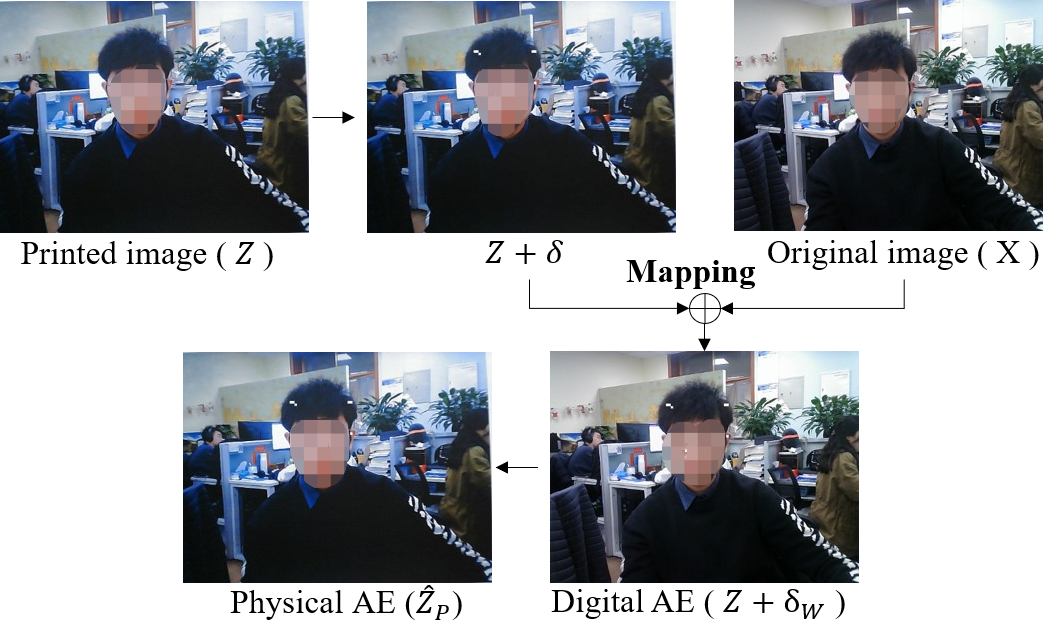
\includegraphics[width = 0.45\textwidth]{figures/adv_map.png}}
%	\vspace{-0.15in}
%	\caption{The adversarial  perturbation $\delta$ generated based on the printed photo $Z$ is applied to the original image $X$ to form the digital  adversarial example $\widehat{Z}$,  which is then printed and captured as the physical adversarial photo $\widehat{Z}_p$. }
%	\label{rgb_adv}
%		\vspace{-0.15in}
%\end{figure}

%\textbf{Printed Photo  Calibration. }
%To eliminate the color distortion on the photo part, we use the
%printed photo $Z$ for optimization but apply the generated adversarial perturbations on the original (digital) image $X$ of the printed photo $Z$ to form the adversarial example $\widehat{Z}$. The printed photo $Z$ is the original image $X$ after a printing-capturing process, i.e., $Z=C[P(X)]$. As a result, if we apply the generated adversarial perturbations on the original image $X$ instead of the printed photo $Z$, the adversarial photo $\widehat{Z}_p$ becomes as follows:
%\begin{equation}
%	\widehat{Z}_p=C[P(X+\delta)] =C[P(X)]+C[P(\delta)]= Z + C[P(\delta)]\label{rgb_3}
%\end{equation}
 %An illustration is shown in Fig.~\ref{rgb_adv}, where we first capture the legitimate user's image as $X$, and then print $X$ out as the printed photo $Z$ (detected as ``Non-living''). Then, we use the printed photo $Z$ to generate adversarial perturbations $\delta$ that can spoof the RGB-based liveness detection, apply it to the origin image $X$ to form the adversarial example $\widehat{Z}$, and  finally print it out as the physical adversarial photo $\widehat{Z}_p$. 
%In this way, we eliminate the color distortion on the photo part.


%\textbf{Perturbation Calibration.} 
%We then calibrate the impacts of printing and capturing for the adversarial perturbation $\delta$. Specifically, we consider reducing its effects from two aspects: (1) perturbation color, and (2) perturbation size. 


%Adversarial perturbations areusually of various colors, resulting in severe color distortions during the printing-captioning process. 
%Using a color that suffers from fewer color shifts in both the printing and capturing process can help enhance the robustness of the generated adversarial perturbations.
%To achieve it, we analyze the commonly-used color mode of the printer, i.e., CMYK~\cite{yin2013image}, and find that in this color mode, white  is represented as 0 cyan, 0 yellow, 0 magenta, and 0 black. As a result, using the color white to generate adversarial perturbations is likely to reduce the color distortion caused by the printing. Moreover, since the white color reflects all lights and thus may also suffer from the least distortion during the imaging process. Thus, by generating adversarial perturbations of white, we can get a desired adversarial photo as follows :

%\begin{equation}
%	\widehat{Z}_p=C[P(X+\delta)] = Z + \delta
%\end{equation}

%Despite reducing the impacts of printing and capturing by using white adversarial perturbations, increasing the size of each perturbation can also help improve its robustness in the real world.
%The reason is that pixel-level adversarial perturbations are too subtle to survive from noises introduced by the  printing-capturing process.
%As a result, we use a square instead of a pixel as the basic unit of the adversarial perturbations. Since the face authentication system allows a small portion of the user's face to be obscured, such an operation will not impact face recognition.



